\section{Results}

We can use the uniqueness measure to understand the rate at which new ideas arrive. As we gather more and more ideas in the course of an experiment, we expect that we will see fewer ideas that are not already in our idea pool. Figure FIG shows the cumulative count of ideas as a function of the number of instances gathered in the experiment. To smooth the plot, the order in which instances were received was shuffled 100 times, and the mean of the cumulative unique idea count was taken at each step.

\begin{figure}[h!]
    \centering
    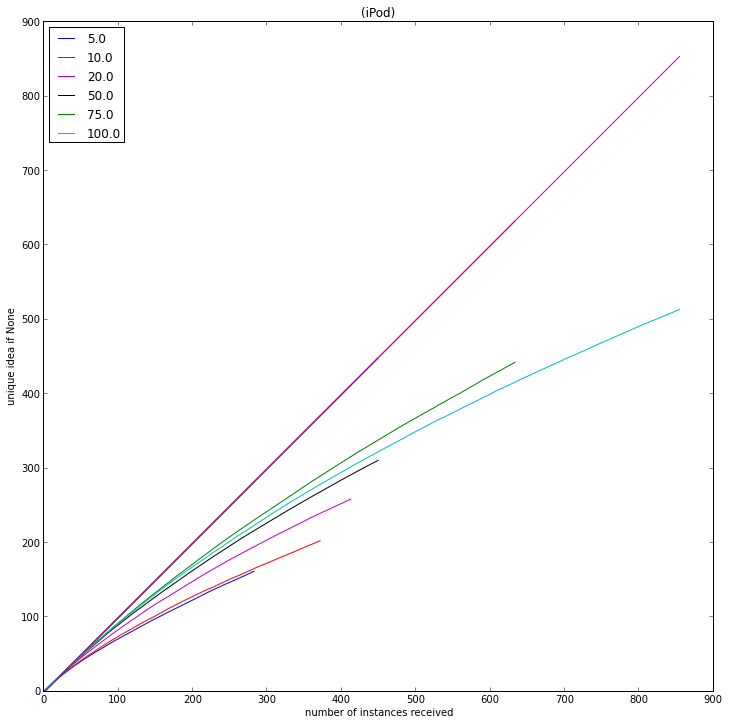
\includegraphics[width=0.9\columnwidth]{ideas_over_time}
    \caption{Cumulative idea count}
\end{figure}

The horizontal line in Figure FIG represent the idea case, in which each instance represents a different idea (i.e. every answer we receive is a new, unique idea). As expected, the rate at which ideas are gained appears to taper off.

Figure FIG more closely examines the rate, the primary property of interest. The panels, from top to bottom, are the rate at which new ideas, categories, and non-singleton categories are generated, respectively. Similar to Figure FIG, these are based on shuffling the order of instances 10000 times and taking the mean of the derivative at each point. In this case, the ideal (a 1:1:1 instance:idea:category ratio) is represented by the horizontal bar across the top of the chart.

\begin{figure}[h!]
    \centering
    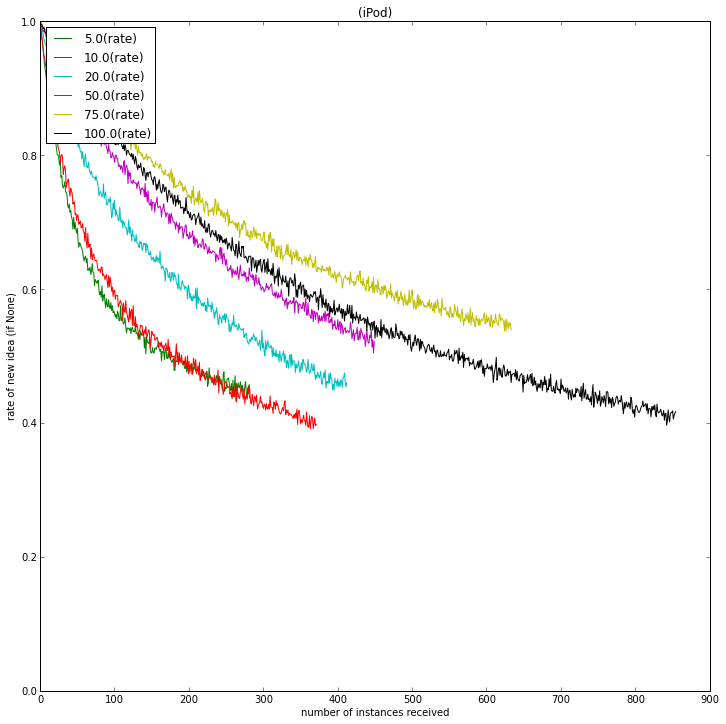
\includegraphics[width=0.7\columnwidth]{rate_new_idea_over_time}
    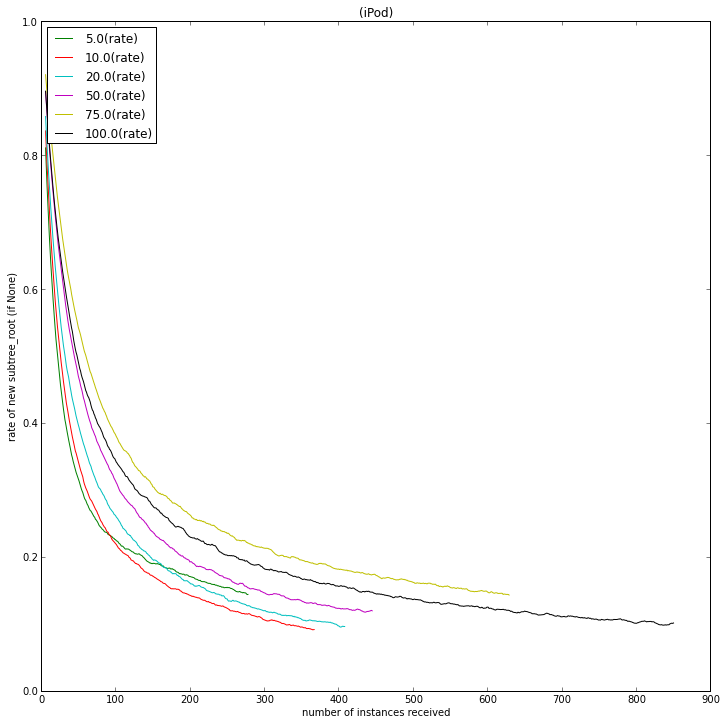
\includegraphics[width=0.7\columnwidth]{rate_new_category_over_time}
    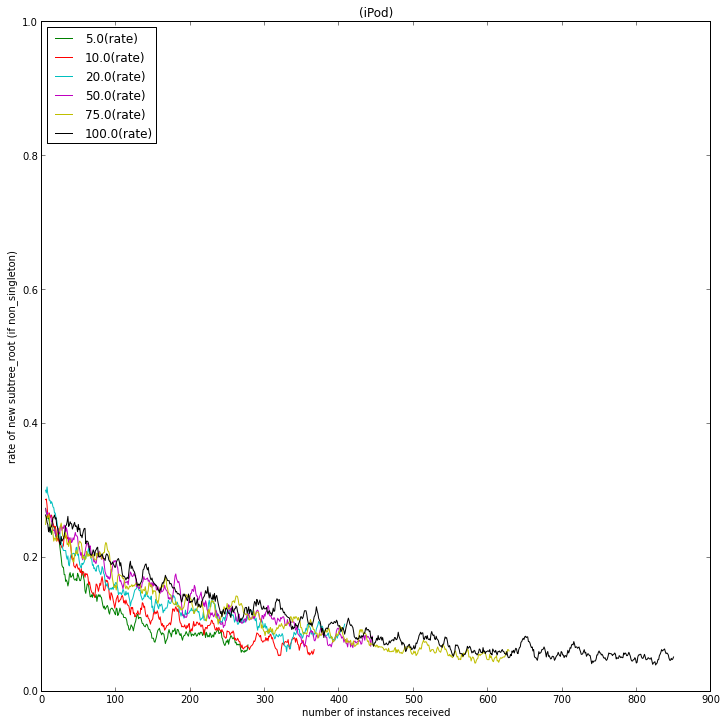
\includegraphics[width=0.7\columnwidth]{rate_new_ns_category_over_time}
    \caption{Rate of idea generation}
\end{figure}

The number of ideas, categories and non-singleton each drop off exponentially over time. It is unsurprising that the number of new categories should drop off faster than the number of new ideas, as we expect that there are fewer categories of ideas than there are individual ideas themselves.

The third panel, which shows non-singleton categories over time, tells a distinctly different story from the others. While in the idea and category plots, the height-ordering of rates of generation between categories remains generally identical, there is a point of intersection and reversal in the non-singleton category plot at around the 30 instances point. Before this point, the lower conditions actually generate new categories at a \emph{faster} rate.

In lower conditions, brainstormers will quickly offer up big, popular, non-singleton categories. Beyond the inflection point, the category pool is saturated with these low-hanging fruit, and only brainstormers tasked with generating more ideas will find the smaller category. This is a more nuanced view of the tree node/instance quartiles in Section SEC; condition 5 brainstormers cover the spectrum of category sizes while condition 100 brainstormers pull from the smaller category trees in the forest.

\subsubsection{Hypothesis 1}

Visually, the rate of idea, category and singleton category generation seems to trend towards 0. We tested this hypothesis...

Additionally Figure FIG indicates that there is some effect of number of ideas requested on the rate of generation. Generally, conditions with more requested responses generated ideas and categories at a higher rate.

Test here...

\subsubsection{Hypothesis 2}

Test here...

\subsection{Originality}

We measure differences in originality between conditions by examining the idea o-score and category o-score. The distributions of these scores are summarized in Figure FIG. The left panel compares idea o-score and the right compares category o-score.

\begin{figure}[h!]
    \centering
    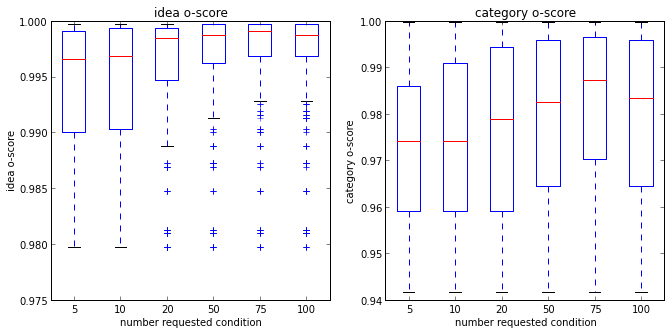
\includegraphics[width=0.9\columnwidth]{oscores_conditions}
\end{figure}

The more ideas requested, the more original the ideas produced. As suggested by the instance quartile range in section SEC, higher number conditions produce idea in trees with fewer instances, thus the high category o-score. We also see that these conditions produce \emph{ideas} with fewer instances.

As the originality rises, however, so does the number of outliers. To understand this phenomenon, we need to more closely observe the distribution of originality scores between not just conditions, but ordinal position in a brianstorming run.

Figure FIG provides this visualization. The upper panel gives the mean idea o-score as a function of ordinal position in all 100 condition brainstorming runs. The o-score for each ordinal position is the mean of all idea o-scores for that ordinal position in a run. Following this, the plot is further smoothed by making each point the mean of a sliding window of size 10 around its ordinal position. The bottom panel is a similar plot for category-oscore. To aid in interpretation, the first, second and third quartiles are also represented on the plot. The error bars are standard error.

\begin{figure}[h]
    \centering
    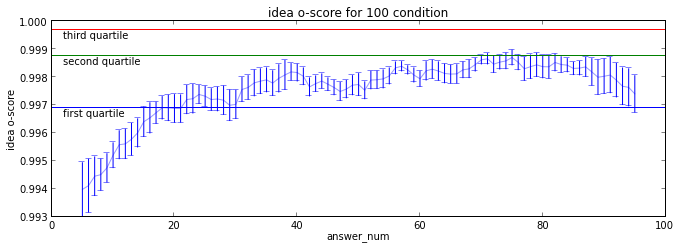
\includegraphics[width=0.9\columnwidth]{idea_oscore_order_100}
    \caption{Idea o-score as a function of order (100 condition)}
    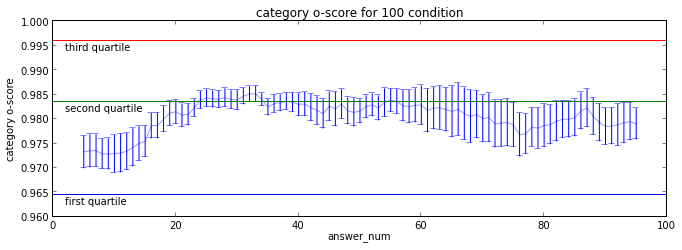
\includegraphics[width=0.9\columnwidth]{cat_oscore_order_100}
    \caption{Category o-score as a function of order (100 condition)}
\end{figure}

The only part of the originality score that falls outside the first and third quartiles is the beginning of the run. Participants in the higher numbered conditions generate more original ideas overall, but not until they have exceeded some threshold of common ideas. Figure FIG replicates figure FIG but across all conditions, and the same pattern of originality growth until an originality peak - around 20 ideas - is reached. Note that because of the additional HITs, there are far more examples of early-order ideas in the 5, 10 and 20 conditions than in the 50, 75, or 100, so this pattern is present without any dominating affect by the upper conditions.

\begin{figure}[h]
    \centering
    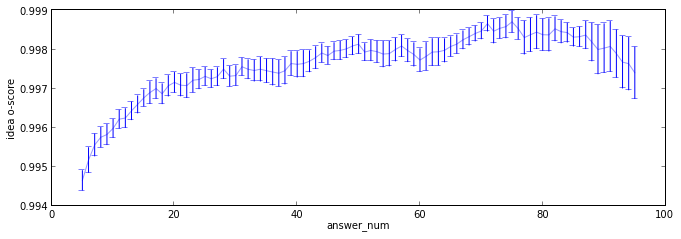
\includegraphics[width=0.9\columnwidth]{idea_oscore_order}
    \caption{Idea o-score as a function of order}
    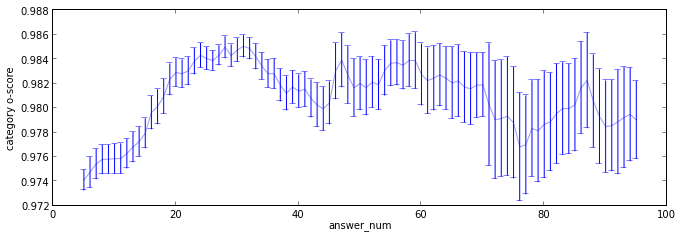
\includegraphics[width=0.9\columnwidth]{cat_oscore_order}
    \caption{Category o-score as a function of order}
\end{figure}

A similar, although less severe, pattern is observed for category o-score. There is a gradual increase in category originality until the 20 instance threshold is reached, at which point variance of the scores increases rapidly and no clear pattern is observable. This is explained by the relationship between common ideas and common categories. We expect that unoriginal ideas belong to unoriginal categories, as a high instance count for an idea increases the instance count for its category tree. However, we cannot make the inverse assumption, that a high originality idea belongs to a high originality category. Once the common idea are exhausted, then, there is no relationship between idea originality and category originality.

\subsubsection{Hypothesis 6}

This threshold at 20 ideas brings us to \textbf{Hypothesis 6:} Ideas generated in the latter half of a brainstorming session are of higher originality than ideas generated in the former half. With our empirical evidence, we can instead test that ideas \emph{more than 20 instances into a brainstorming session} are more original than those in the first 20 instances, regardless of condition.

Test here...

\subsection{Riffing}


\subsubsection{SIAM hypotheses}

\cite{nijstad_how_2006}